\section{State of the art}

Before introducing the state of the art let us discuss a bit the physical realization of qubits.
\subsection{Different qubit implementations}

At the time of writing there are currently two technologies for implementing qubits:
\begin{itemize}
\item Trapped ions.
\item Superconducting circuit.
\end{itemize}

Let us focus on the type of qubit used in the machine we are going to use:
\paragraph{Superconducting qubits}
To create a solid-state qubit, like any other kind of qubit, we need to isolate a two-level quantum system. To date, efforts to make solid-state qubits have focused on superconductors and semiconductors. While interesting results have been obtained with two semiconductor approaches, quantum dots and single-donor systems, the superconducting approach is currently the most advanced.

To maintain coherence it is essential to keep electron-electron interactions, and also interactions between electrons and other degrees of freedom (such as phonons in the solid), under control. Superconductors have the advantage in this regard because the electrons condense into Cooper pairs that form a single superfluid. This superfluid is able to move through the metal lattice without any resistance (i.e. without interactions) because it takes a certain amount of energy, known as the energy gap, to break up the Cooper pairs.

In aluminum, a popular material for making superconducting quantum circuits, the energy gap corresponds to a frequency of 90 GHz at a temperature of 20 mK. This gap is an order of magnitude greater than the typical energy difference between the two levels in a superconducting qubit, which means that we can “drive” the qubit without breaking up the Cooper pairs and jeopardizing the quantum coherence of the system.

The behavior of the electron superfluid is completely determined by a single quantum wavefunction. The amplitude of this wavefunction determines the number of Cooper pairs, while the value of the phase is related to the supercurrent and any magnetic field that is present. The amplitude and phase of the wavefunction are conjugate variables, that is, they are related by an uncertainty principle that means we cannot measure both of their values with arbitrary precision at the same time. 

The two primary types of superconducting qubit, the charge qubit and the flux qubit, are directly related to these two variables: charge qubits are associated with the amplitude, while flux qubits are related to the phase. \cite{Supercon84:online}

\subsubsection*{State of the art}

In figure~\ref{fig:state-of-the-art} we report a summary of state-of-art experimental digital quantum simulations from~\cite{UQC}. Open circles represent results obtained on superconducting circuits quantum processors, while squares correspond to experimental quantum simulations on trapped ions processors. The color code corresponds to different target models being simulated\footnote{They are simply different Hamiltonian: their description would be redundant and it is purposely skipped, in chapter~\ref{chap:3} we are going to describe our Hamiltonian of interest.}: two-spin Transverse field Ising model $\left(\mathrm{TIM}_{2}\right)$, two-spin XY $\left(\mathrm{XY}_{2}\right)$ and $\mathrm{XYZ}\left(\mathrm{XYZ}_{2}\right)$ models, 3- and 6-spin many body interactions, two-spin Heisenberg model (Heis ${ }_{2}$), and 2to 4 -mode Fermi Hubbard model $\left(\mathrm{FH}_{x}\right.$, with $\left.x=2,3,4\right)$.

As we are going to see in chapter~\ref{chap:3} Jakarta (the device used in our experiments) is using superconducting Qubits, specifically the \emph{Transmon}. The description of the Transmon is way beyond the scope of this work but you can find more info on that here~\cite{Transmon}.

We are interested, as again we are going to see in chapter~\ref{chap:3}, to two-spin Heisenberg model (Heis ${ }_{2}$). That means that the state of the art is around 0.7 in our case\footnote{Why? Again wait for chapter~\ref{chap:3}, the problem limit us to four steps of trotterization.}.

It is very interesting to see that accuracy seems to decrease with trotterization steps. Why? According to the formula of chapter~\ref{chap:2} it should be exactly the opposite! We are speculating here as there are no known source proving this but our guess is that increasing the number of trotterization steps increase the circuit and thus increase noise in the simulation. This seems a reasonable explanation and it is the reason why we will limit ourself in the number of steps.
\begin{figure}[htb]
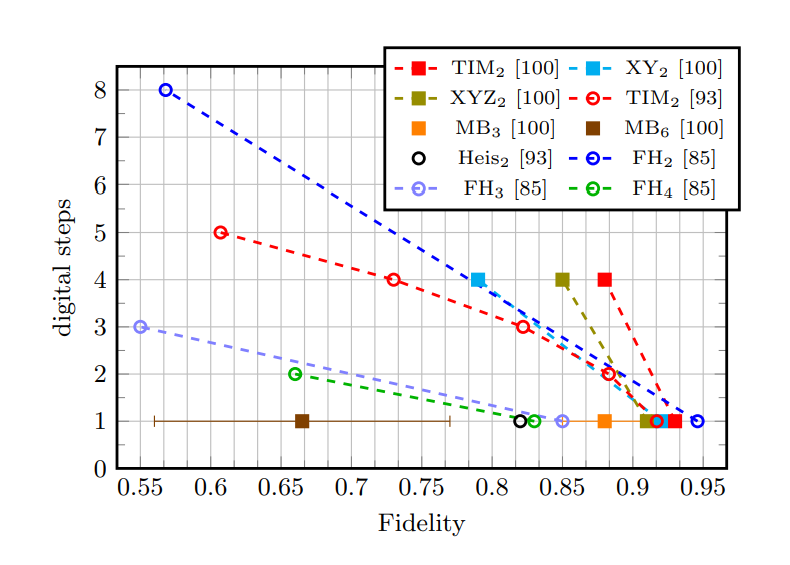
\includegraphics[width=1.25\textwidth]{state-of-the-art.png}
\centering
\caption{State of the art}
\label{fig:state-of-the-art}
\end{figure}


